	\newpage	
	\center{\section{Постановка задачи}}
	
	
	\flushleft{Реализовать алгоритмы умножения матриц:}
	\begin{enumerate}
		\item Стандартный
		\item Винограда
		\item Улучшенного Винограда
	\end{enumerate}
	Рассчитать сложность алгоритмов и провести временные эксперименты
	
	\center{\section{Модель вычислений}}
	\flushleft
	Операнды +, -, *, /, <, >, <=, >=, ==, !=, [ ] имеют значение f = 1;\\
	Значение для цикла f = 2 + N(...), где N - количество итераций.
	
	

%%%%%%%%%%%%%%%%%%%%%%%%%%%%%%
	
	\newpage
	\center{\section{Блок-схемы}}
	\begin{figure}[h!]
		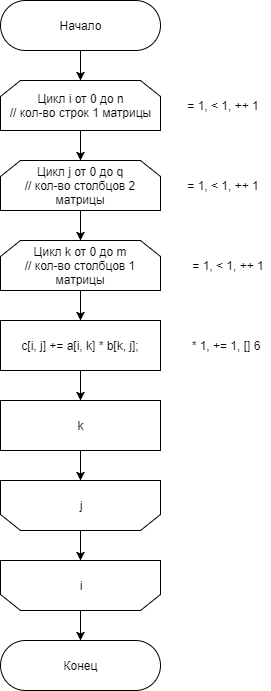
\includegraphics[width=0.5\linewidth]{usual_bs.png}
		\caption{Блок-схема базового алгоритма}
	\end{figure}
	
	\newpage
	\begin{figure}[h!]
		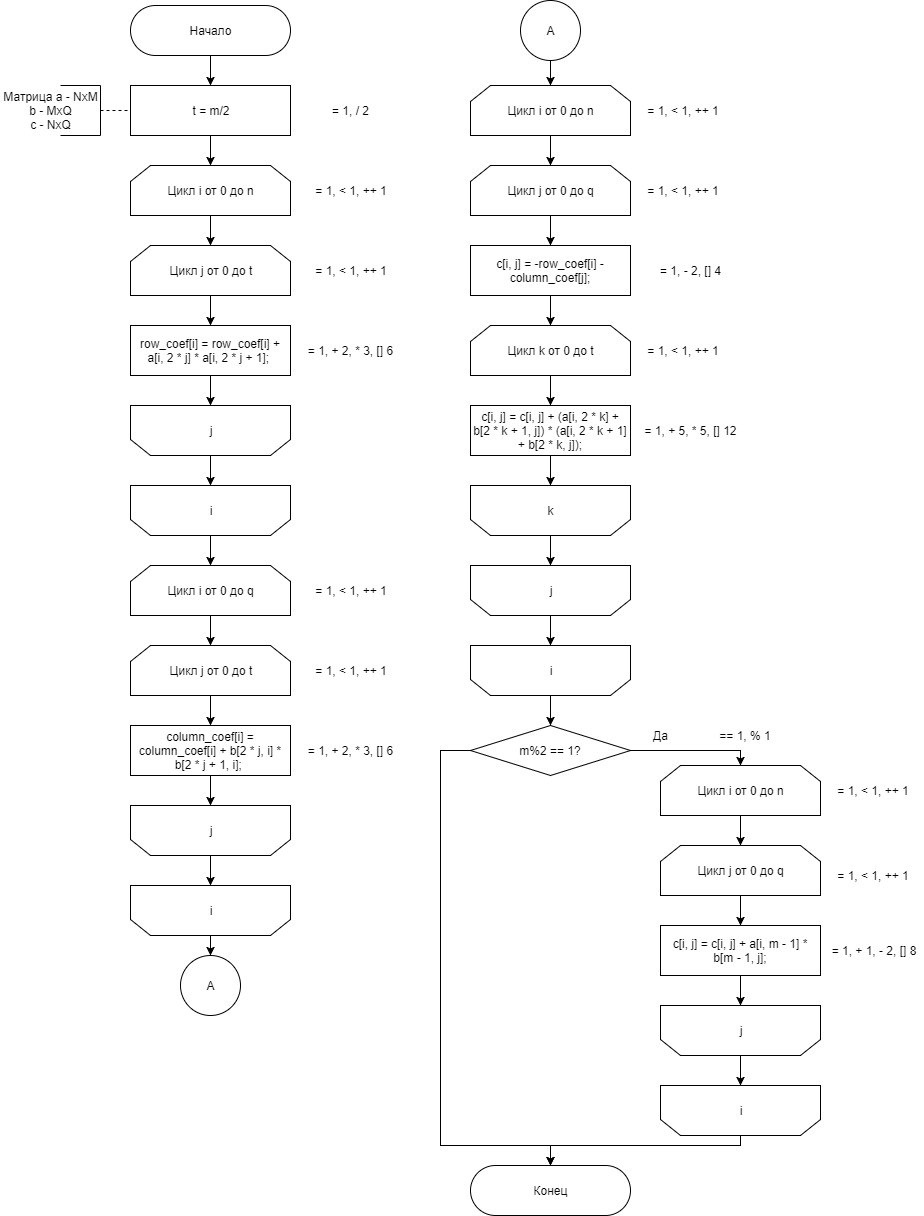
\includegraphics[width=1.05\linewidth]{Vinograd_bs.png}
		\caption{Блок-схема алгоритма Винограда}
	\end{figure}

	\newpage
	\begin{figure}[h!]
	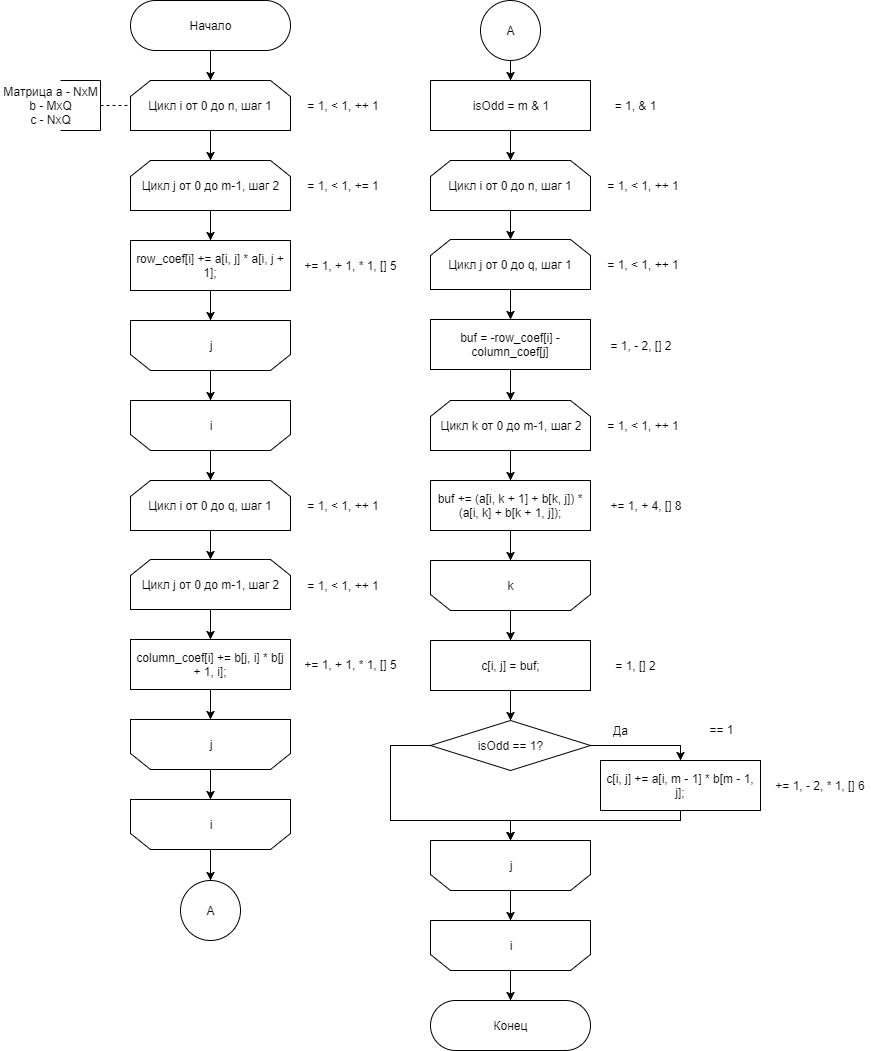
\includegraphics[width=1.05\linewidth]{Vinograd_B_bs.png}
	\caption{Блок-схема улучшенного алгоритма Винограда}
	\end{figure}



%%%%%%%%%%%%%%%%%%%%%%%%%%%%%%

	\newpage
	\center{\section{Листинг}}
	
	\textbf{\textsc{main.cpp:}}
	\lstset{breaklines=true, numbers=left,
		 keywordstyle=\color{blue}, commentstyle=\color{red}}
	\lstinputlisting[language=c++]{../Mat/main.cpp}
	
	\vspace{\baselineskip}
	
	\textbf{\textsc{mymat.cpp:}}
	\lstset{breaklines=true, numbers=left,
		keywordstyle=\color{blue}, commentstyle=\color{red}}
	\lstinputlisting[language=c++]{../Mat/mymat.cpp}	
	

%%%%%%%%%%%%%%%%%%%%%%%%%%%%%%	


	\newpage
	\center{\section{Временные  эксперименты  }}
	
	\flushleft
	Измерения проводились для квадратных вещественных матриц
	
	\begin{center} % makecell нужен для разрыва строки в ячейках -- \\ разрыв для всей таблицы
		\begin{tabular}{|c|c|c|c|}
			\hline
			Размеры матриц & Обычное & Виноград & Улучшенный Виноград\\
			
			\hline 
			100x100 & 
			24.6549 & 
			14.0676 &
			11.3303\\
			
			
			\hline 
			200x200 & 
			170.8249 &
			137.3591 &
			119.8764 \\
			
			\hline 
			300x300 & 
			488.6610 &
			429.6541 &
			355.9341 \\
			
			
			\hline 
			400x400 & 
			1358.2967 &
			1082.4930 &
			935.0479 \\
			
			
			\hline 
			500x500 & 
			3132.0469 &
			2562.7789 &
			2248.1820 \\
			
			\hline 
			600x600 & 
			5765.4314 &
			4467.8990 &
			3802.2509 \\
			
			\hline 
			700x700 & 
			8566.0461 &
			7090.2327 &
			6045.3397 \\
			
			\hline 
			800x800 & 
			12530.9540 &
			10513.3806 &
			9130.0609 \\
			
			\hline 
			900x900 & 
			18801.5250 &
			15415.6954 &
			13241.0050 \\
			
			\hline 
			1000x1000 & 
			26042.9380 &
			24677.6349 &
			26579.2120 \\
			
			\hline			
		\end{tabular}
	\end{center}
	
	\center{\textsc{Замеры времени в милисекундах (среднее из 7 замеров)\\}}
	
	\newpage
	
	\begin{figure}[h!]
		\center{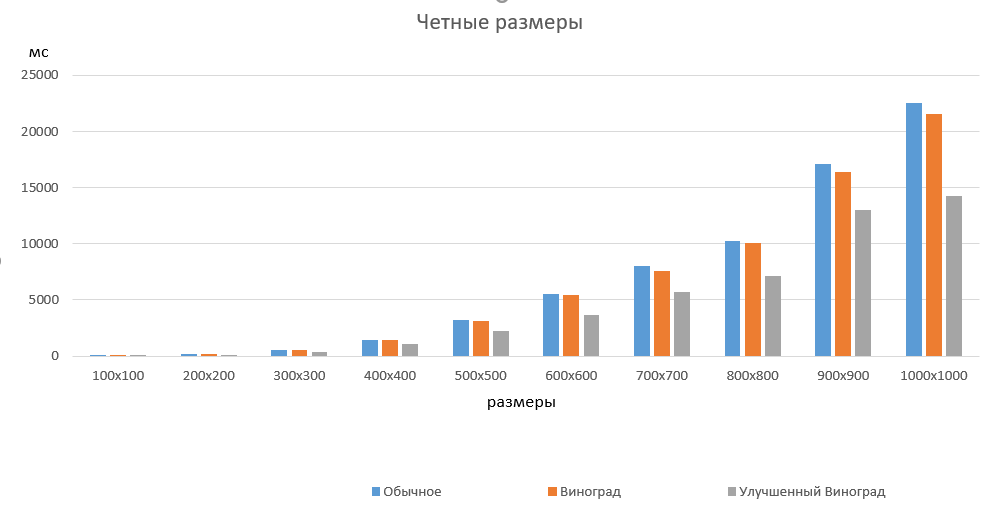
\includegraphics[width=\linewidth]{4et}}
		\caption{Сравнение времени при четном кол-ве элементов}
		
		\hfill
		
		\center{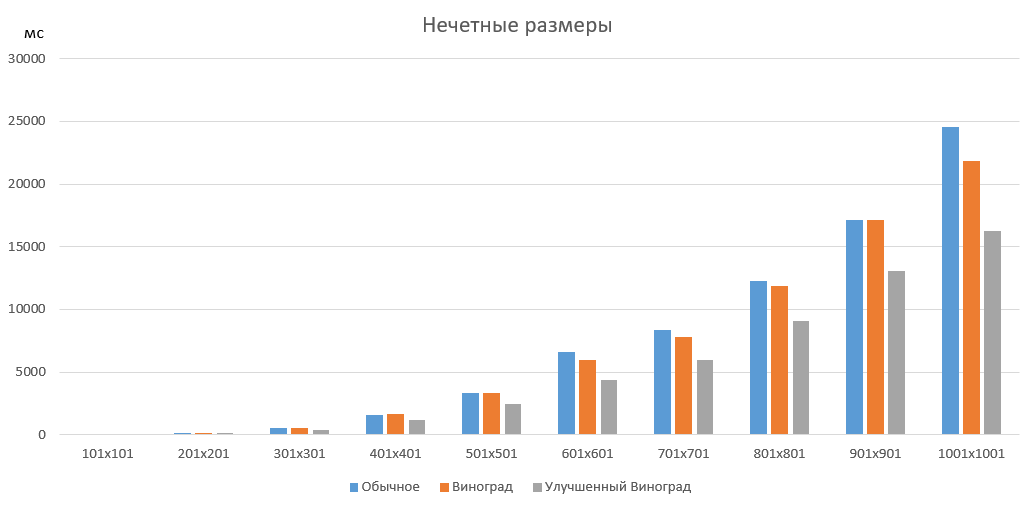
\includegraphics[width=\linewidth]{ne4et}}
		\caption{Сравнение времени при нечетном кол-ве элементов}
	\end{figure}

%%%%%%%%%%%%%%%%%%%%%%%%%%%%%%		

	\newpage
	\section{Теоретическая оценка }
	\flushleft
	а) Обычное умножение:\\
	$f = 2+N*(2+2+Q(2+2+M(2+8))) = 2+4N+4NQ+10MNQ \sim O(n^3)$
	
	б) Умножение алгоритмом Винограда:
	\begin{itemize}
		\item Переменная t: $f = 2$
		\item row coef: $f = 2+N(2+2+2+M/2(2+12)) = 2+6N+7MN$
		\item column coef: $f = 2+Q(2+2+2+M/2(2+12)) = 2+6Q+7MQ$
		\item Вычисление результирующей матрицы: $f = 2+N(2+2+Q(2+7+2+M/2(2+23))) = 2+4N+11QN+25MNQ/2$
		\item Вычисления последней строки: $f = 2+2+N(2+2+Q(2+13)) = 4+4N+15NQ$ 
	\end{itemize}
	Лучший случай (размер матрицы четный): $f = 2+2+6N+7MN+2+6Q+7MQ+2+4N+11QN+25MNQ/2 = 8+10N+7MN+6Q+7QM+11QN+25QMN/2 \sim O(n^3)$\\
	Худший случай (размер матрицы нечетный): $f = 2+2+6N+7MN+2+6Q+7MQ+2+4N+11QN+25MNQ/2+4+4N+15NQ = 12+14N+7MN+6Q+7QM+26QN+25QMN/2 \sim O(n^3)$\\
	
	в) Умножение улучшенным алгоритмом Винограда:\\
	\begin{itemize}
		\item Переменная t: $f = 2$
		\item row coef: $f = 2+N(2+2+2+(M-1)/2(2+8)) = 5MN+N+2$
		\item column coef: $f = 2+Q(2+2+2+(M-1)/2(2+8)) = 5MQ+Q+2$
		\item Переменная isOdd: $f = 2$
		\item Вычисление результирующей матрицы: $f = 2+N(2+2+Q(2+5+2+(M-1)/2(2+14)+3[+1+10])) = 2+4N+8MNQ+[5NQ|14NQ]$
	\end{itemize}
	Лучший случай (размер матрицы четный): $f = 2+5MN+N+2+5MQ+Q+2+2+2+4N+8MNQ+5NQ = 10+Q+5N+5MN+5MQ+5NQ+8MNQ \sim O(n^3)$\\
	Худший случай (размер матрицы нечетный): $f = 2+2-4N+10MN+2-4Q+10MQ+2+2+4N+8MNQ+13NQ = 10+Q+5N+5MN+5MQ+13NQ+8MNQ \sim O(n^3)$\\
	\flushleft
	
		
			
%%%%%%%%%%%%%%%%%%%%%%%%%%%%%%		
	
	\newpage
	\center{\section{Выводы}}
	\flushleft

	Сравнение алгоритмов по времени подтверждает теоретические замеры времени. Алгоритмы работают примерно одинаково, что подтверждает их оценка трудоемкости порядка $O(n^3)$.
	
	После умножения матриц размерами примерно 600х600 алгоритм Винограда работает быстрее обычного алгоритма умножения матриц постоянно.
	
%%%%%%%%%%%%%%%%%%%%%%%%%%%%%%	
	
	\newpage
	\center{\section{Заключение}}
	
	
	\flushleft
	В ходе лабораторной работы были реализованы 3 алгоритма умножения матриц: классический, алгоритм Винограда и улучшенным алгоритмом Винограда. Были получены навыки работы с матрицами и контейнером std::vector в C++, а так же с \LaTeX. Изучен подход к вычислению сложности алгоритмов.